\chapter{IQM Selection Strategy: Linking Ratings to Image Features}
\label{chap:iqm_selection_strategy}

Identifying the most effective image quality indicators, i.e. IQMs, for a machine learning model to differentiate between good and poor quality images is a crucial step in this project. This step relies on the analysis of manually assessed images and their associated artifact scores to highlight correlations between visual features and perceived quality. This chapter first details the reliability of the manual scoring process by analyzing the consistency of human assessments by raters. It then discusses the influence of various image artifacts on these human quality judgments. Finally, it describes the strategic selection of IQMs, informed by both statistical analysis and visual features observed in different image quality classes.

\section{Analysis of Artifact Influence on Image Quality Ratings}
\label{sec:analysis_artifact_influence}

To effectively select relevant IQMs to train a good and bad quality classification model, we must first understand what factors determine image quality. To do this, there are two key steps
\begin{enumerate}
    \item \textbf{Ensuring Inter-Rater Reliability:} Confirm the consistency of the evaluators' assessments. It is necessary to ensure that they are able to distinguish a good image from a bad one.
    \item \textbf{Identifying Impactful Artifacts:} Determine the specific image artifacts that most impacted their overall quality judgments. This allows IQMs to be prioritized to the most critical types of degradation.
\end{enumerate}

\subsection{Establishing Inter-Rater Reliability: How Consistent Are The Raters?}
\label{sec:inter_rater_reliability}

Before using manual image ratings as a benchmark for IQM selection, it is essential to confirm that our three expert raters applied the quality criteria consistently. If their agreement is low, the ratings are less reliable as a "ground truth." This section assesses this consistency using several standard statistical measures and provides an initial overview of rating distributions.

\subsubsection{Initial Rater Distribution Analysis}
\label{sssec:initial_rater_distribution}

First, a pie chart was generated to visualize the distribution of ratings assigned by each expert rater. This provides an initial insight into how frequently each rater assigned images to different quality categories, hinting at potential inter-rater variability before formal statistical assessment

\begin{figure}[htbp]
    \centering
    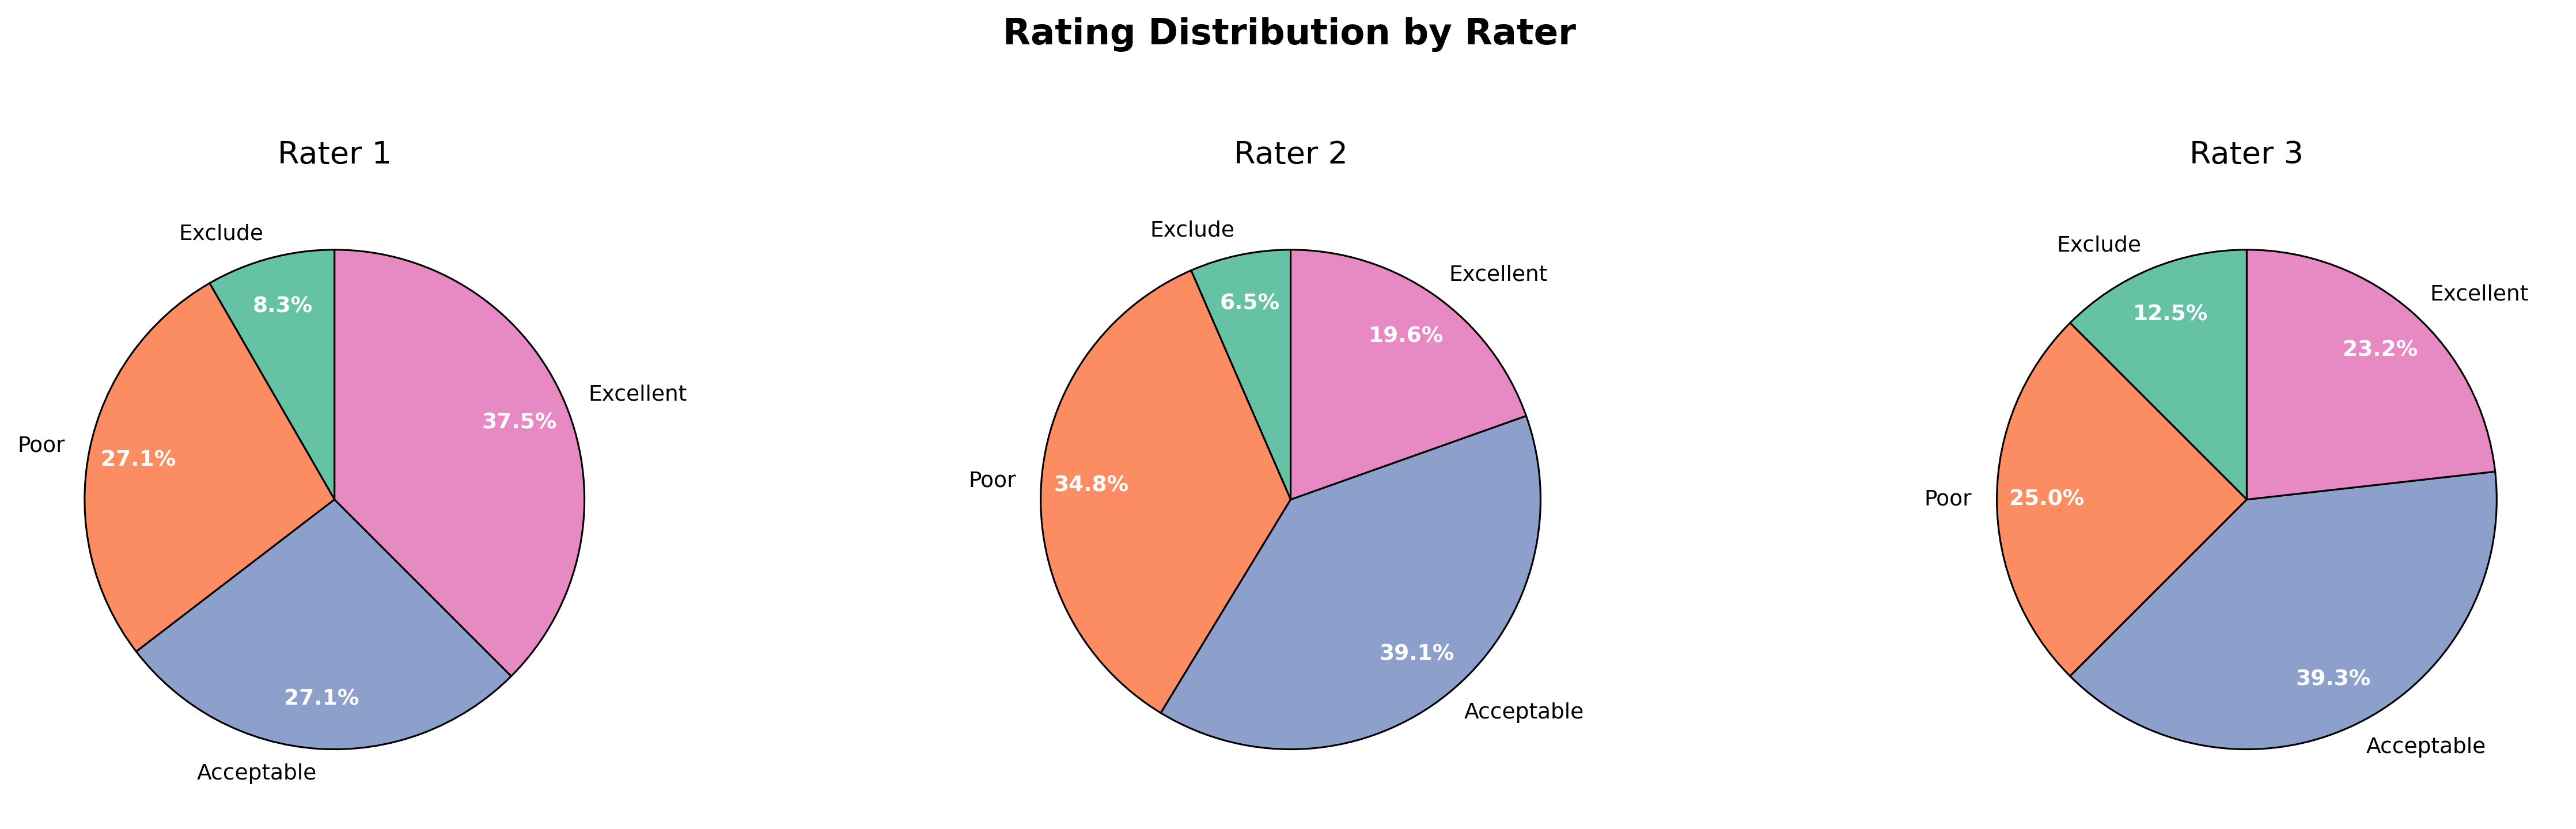
\includegraphics[width=0.9\linewidth]{Report/img/rating_by_rater_pie.png}
    \caption{Rating distribution by rater across 'Exclude', 'Poor', 'Acceptable', and 'Excellent' categories. Note the variations in how frequently each rater assigned images to the different quality categories. Figure from others degradation are in \ref{app:distribution}.}
    \label{fig:rating_distribution_by_rater}
\end{figure}

As shown in Figure~\ref{fig:rating_distribution_by_rater}, analysis of image quality ratings reveals significant inter-rater variability across the four defined categories: “Exclude,” “Poor,” “Acceptable,” and “Excellent.” This demonstrates, first of all, the difficulty of manually classifying image quality. This already represents a challenge for the project. A key observation is the varying rigor between raters. Rater 3, for example, displayed the strictest rating trends, classifying 12.5\% of images as “Exclude.” This percentage is significantly higher than that of Rater 1 (8.3\%), and is nearly double the proportion designated by Rater 2 (6.5\%) for the same critical category. Conversely, Rater 1 showed the greatest tolerance for good quality images, rating 37.5\% of images as “Excellent,” compared to 19.6\% for Rater 2 and 23.2\% for Reviewer 3.

Overall, differences are discernible in how each rater interprets the quality assessment criteria. This variability may pose a challenge when training the model.

\subsubsection{Inter-Rater Reliability Assessment Methodology}
\label{sssec:irr_methodology}
To quantitatively assess the consistency between the three raters, two statistical measures are calculated for each image quality measure assessed (see the Metric column in Table \ref{tab:irr_results_actual}):
\begin{itemize}
    \item \textbf{Intraclass Correlation Coefficient (ICC):} Specifically, the ICC(A,k) is used to assess the agreement of the average measurements of $k=3$ raters. This coefficient indicates the consistency with which raters rated the images on a continuous scale [0-4]. Values close to 1 indicate higher agreement, with an ICC coefficient > 0.75 generally considered good to excellent reliability. \textbf{add reference}
    \item \textbf{Percentage Agreement:} For the 'Eyes Open Status', a simple percentage agreement was also determined, representing how often all three raters assigned the exact same category.
\end{itemize}

\subsubsection{Inter-Rater Reliability Assessment Results}
\label{sssec:irr_results}

The results of this reliability analysis are summarized in Table~\ref{tab:irr_results_actual} and further illustrated by the correlation matrices in Figure \ref{fig:cm_all_raters_rc}.

\begin{table}[htbp]
\centering
\caption{Inter-Rater Reliability Metrics for Image Quality Assessments}
\label{tab:irr_results_actual}
\resizebox{\textwidth}{!}{
\begin{tabular}{lcccc}
\toprule
\textbf{Metric} & \textbf{ICC(A,k)} & \textbf{ICC CI95\% Low} & \textbf{ICC CI95\% High} & \textbf{\% Agreement} \\
\midrule
rating          & -0.149   & -1.490          & 0.520           & -            \\
rating1         & 0.144    & -0.820          & 0.640           & -            \\
rating2         & -0.293   & -1.800          & 0.460           & -            \\
blur            & -0.289   & -1.510          & 0.430           & -            \\
noise           & -0.404   & -1.960          & 0.400           & -            \\
motion          & 0.136    & -0.800          & 0.630           & -            \\
bgair           & -0.328   & -2.020          & 0.450           & -            \\
Eyes Open Status& -        & -               & -               & 40.000       \\
\bottomrule
\end{tabular}
} 
\end{table}

%\paragraph{Interpretation of Continuous Ratings (ICC)}
The intraclass correlation coefficient values for overall quality assessments (“rating”, “rating1”, “rating2”) and specific artifact scores (“blur”, “noise”, “motion”, “bgair”) are consistently low, often negative. For example, “rating” yielded an ICC(A,k) of -0.149 (95\% CI: [-1.490, 0.520]), and “noise” an ICC of -0.404 (95\% CI: [-1.960, 0.400]). According to common interpretation guidelines \cite{koo_guideline_2016}, ICC values below 0.5 indicate low reliability. The resulting ICC values, many of which are negative or close to zero, and their wide 95\% confidence intervals, suggest a lack of consistency among raters when assessing these measures on a continuous scale.
For the "Eyes Open State" measure, the percentage agreement is 40.00\%. This relatively low agreement further highlights the difficulty of obtaining consistent manual assessments.

Overall, the inter-rater reliability analysis consistently indicates low agreement between the three raters for the majority of image quality indicators assessed. This low reliability suggests the difficulty of systematically applying the evaluation criteria and the difficulty of having an accurate ground truth.


\begin{figure}[htbp]
    \centering
    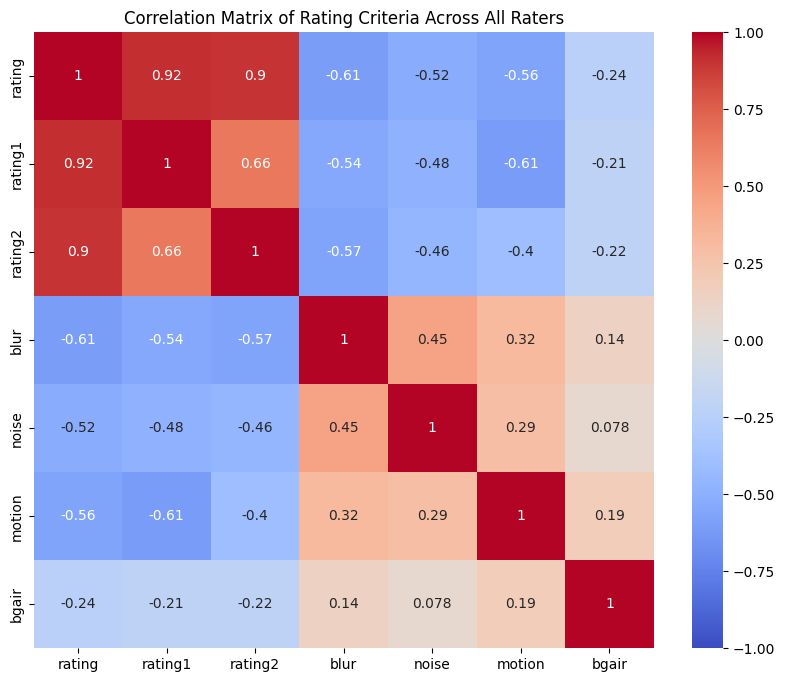
\includegraphics[width=0.5\textwidth]{Report/img/CM_of_all_raters_RC.png}
    \caption{Correlation Matrix of rating criteria across all raters}
    \label{fig:cm_all_raters_rc}
\end{figure}


Impact of Blur on Overall Rating: The artifact exhibiting the strongest correlation with our aggregate image quality rating is blur, with a coefficient of -0.61. This indicates a substantial inverse relationship: as the perceived blur increases, the overall image quality rating tends to decrease significantly.

Inter-Artifact Correlation (Blur and Noise): A moderate positive correlation of 0.45 is observed between blur and noise. This suggests that images high in blur are often also perceived as noisy, potentially reflecting common degradation pathways or the challenge in distinguishing these artifacts during human assessment.


\subsection{Which Image Artifacts Most Impact Human Quality Judgments?}
\label{sec:artifact_impact_lmm}

After assessing the reliability (and limitations) of the manual assessments, the next objective was to identify the specific visual artifacts with the most significant independent influence on overall image quality assessments. Understanding this is essential for prioritizing IQMs sensitive to the most significant image degradations. To achieve this, a Linear Mixed-Effects Model (LMM) was employed. This statistical approach allows for the modeling of the relationship between the overall quality score and the scores of individual artifacts.

\textbf{Key Findings from the LMM:}

The LMM results (summarized in Table~\ref{tab:lmm_results_from_doc}) pinpointed the artifacts that statistically significantly degraded the perceived image quality:

\begin{itemize}
    \item \textbf{Blur:} Showed the \textbf{strongest negative impact}. For each one-unit increase in perceived blur, the overall quality rating decreased by approximately 0.288 ($p < 0.001$).
    \item \textbf{Noise:} Also a significant factor, with each unit increase in noise lowering the quality rating by about 0.254 ($p < 0.001$).
    \item \textbf{Motion:} Had a significant negative effect, reducing the quality rating by roughly 0.204 ($p = 0.001$).
    \item \textbf{Background Artifacts ('bgair'):} In this model, once blur, noise, and motion were accounted for, 'bgair' did not show a statistically significant independent effect on the overall quality rating ($p = 0.089$). While not statistically significant in this specific model, visual reports and qualitative analysis still suggested `bgair` as a relevant factor.
\end{itemize}

\textbf{Implications for IQM Selection:}

The LMM analysis provides clear guidelines for the IQM strategy: Blur, noise, and motion are the main culprits of image quality degradation from the rater's perspective, with blur being the most dominant. Therefore, IQMs must include robust metrics capable of detecting and quantifying these three artifacts. While background artifacts may still be relevant (as suggested by the visual reports and the initial pie chart analysis, Section~\ref{sssec:initial_rater_distribution}), their direct and independent impact on the overall rating appears less critical than the other three when modeled together.

\begin{table}[htbp]
    \centering
    \caption{Simplified Linear Mixed-Effects Model Results (Dependent Variable: rating)}
    \label{tab:lmm_results_from_doc}
    \begin{tabular}{>{\raggedright\arraybackslash}p{2cm}rrrrrr}
    \toprule
        \multicolumn{7}{c}{\textbf{Dependent Variable: rating}} \\
        \textbf{Effect}      & \textbf{Coef.}  & \textbf{Std.Err.} & \textbf{z}       & \textbf{P$>$$|$z$|$} & \textbf{[0.025} & \textbf{0.975]} \\
    \midrule
        Intercept   & 3.081  & 0.106    & 29.159 & 0.000       & 2.874  & 3.288  \\
        blur        & -0.288 & 0.064    & -4.522 & 0.000       & -0.412 & -0.163 \\
        noise       & -0.254 & 0.070    & -3.645 & 0.000       & -0.391 & -0.118 \\
        motion      & -0.204 & 0.061    & -3.313 & 0.001       & -0.324 & -0.083 \\
        bgair       & -0.122 & 0.072    & -1.701 & 0.089       & -0.263 & 0.019  \\
    \midrule
        \multicolumn{7}{l}{\textbf{Random Effect Variance:}} \\
        sub Var     & 0.075  & \multicolumn{2}{l}{(SE: 0.098)} &             &        &        \\
    \midrule
        \multicolumn{7}{l}{\textbf{Model Fit:}} \\
        \multicolumn{7}{p{\dimexpr\linewidth-2\tabcolsep\relax}}{No. Obs: 151, No. Groups: 83, Scale (Residual Var): 0.1809, Log-Likelihood: -115.38} \\
        \multicolumn{7}{l}{Converged: Yes, Method: REML} \\
    \bottomrule
    \end{tabular}
\end{table}

\section{Visual Analysis of Image Quality Classes}
\label{sec:visual_analysis_iq_classes}

In order to refine the selection of IQMs and to complete the statistical results, a qualitative visual evaluation is carried out on images manually classified into three categories: "Excluded", "Poor" and "Excellent". This observation is made on the segmentation carried out for a pre-trained nnU-Net v1 model and 3D images from eye in order to see on which class the model has difficulty segmenting.
\newpage
\subsection{Excluded Images: Severe Degradation}
\label{sec:excluded_images}
Excluded images are characterized by severe degradation, rendering them unusable for analysis. 
\begin{figure}[htbp]
    \centering
    \begin{subfigure}[b]{0.35\textwidth} 
        \centering
        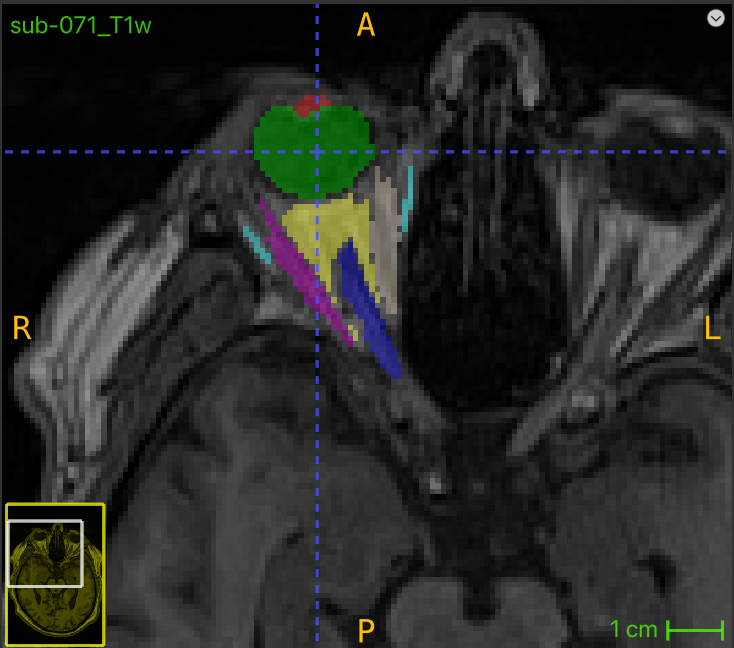
\includegraphics[width=\linewidth]{Report/img/sub-071_T1w.png}
        \caption{T1w - Subject 071}
        \label{subfig:071_T1w}
    \end{subfigure}
    \hspace{0.02\textwidth}
    \begin{subfigure}[b]{0.375\textwidth}
        \centering
        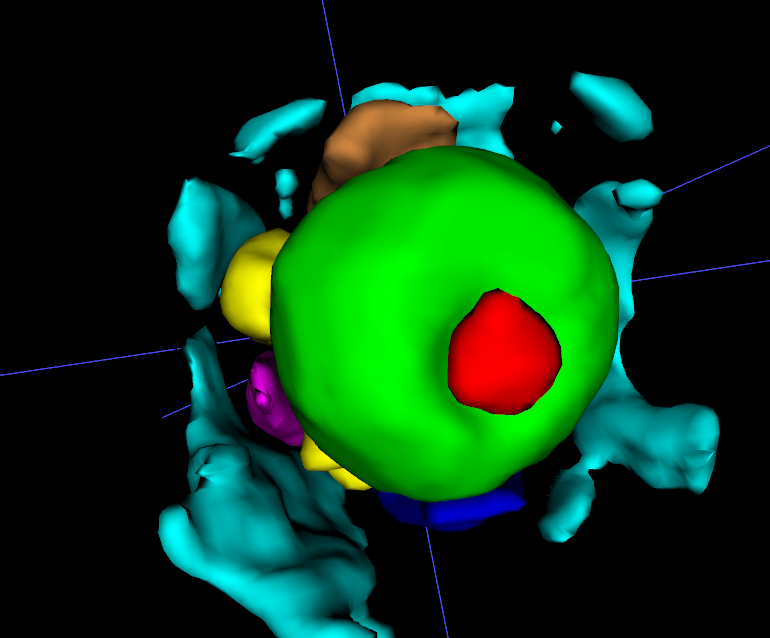
\includegraphics[width=\linewidth]{Report/img/sub-071_T1w_3D.png}
        \caption{T1w\_3D - Subject 071}
        \label{subfig:071_T1w_3D}
    \end{subfigure}

    \vspace{2mm} % Vertical space between rows

    \begin{subfigure}[b]{0.35\textwidth} 
        \centering
        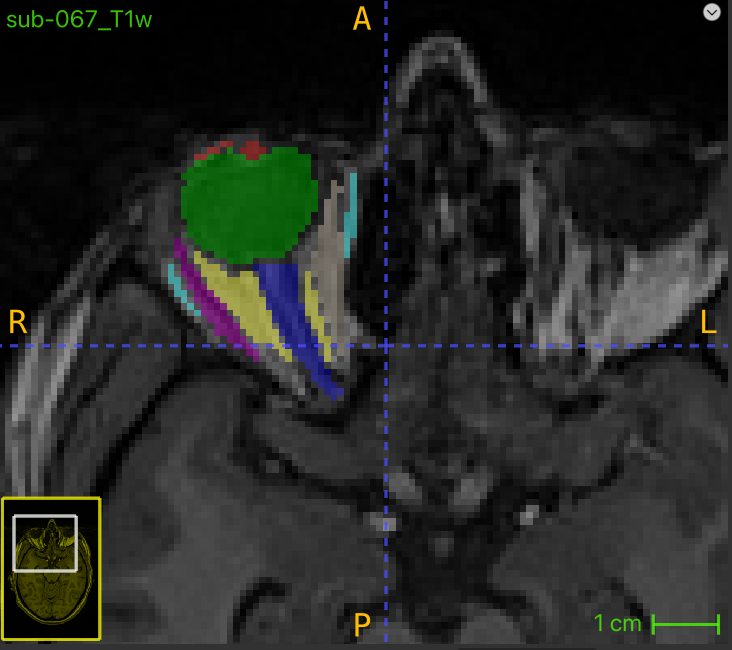
\includegraphics[width=\linewidth]{Report/img/sub-067_T1w.png}
        \caption{T1w - Subject 067}
        \label{subfig:067_T1w}
    \end{subfigure}
    \hspace{0.02\textwidth} 
    \begin{subfigure}[b]{0.375\textwidth} 
        \centering
        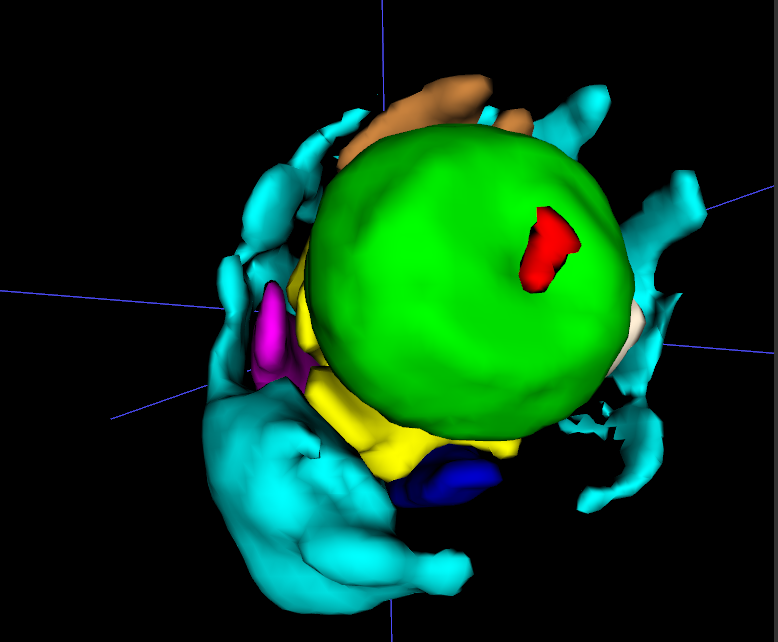
\includegraphics[width=\linewidth]{Report/img/sub-067_T1w_3D.png}
        \caption{T1w\_3D - Subject 067}
        \label{subfig:067_T1w_3D}
    \end{subfigure}
    \caption{Comparison between T1w (left column) and T1w\_3D (right column) images categorized as 'Excluded' quality. These examples demonstrate severe lens segmentation issues, geometric distortions, and general image degradation.}
    \label{fig:excluded_images}
\end{figure}

\subsubsection{Observation}
In the segmented excluded images, severe deficiencies are consistently observed. The lenses are poorly segmented, often deviating significantly from their characteristic ellipsoidal shape. Similarly, the globe segmentation exhibits notable surface imperfections. Furthermore, muscle segmentation frequently contains aberrations, with multiple unrelated pieces being segmented, leading to overall poor quality.
\newpage

\subsection{Bad Quality Images: Noticeable Imperfections}
\label{sec:bad_quality_images}
Images in the "Bad Quality" (poor and acceptable class) category are not necessarily unusable but show noticeable imperfections that distinguish them from excellent quality, yet they are not as severely compromised as "Excluded" images.
\begin{figure}[htbp]
    \centering
    \begin{subfigure}[b]{0.35\textwidth}
        \centering
        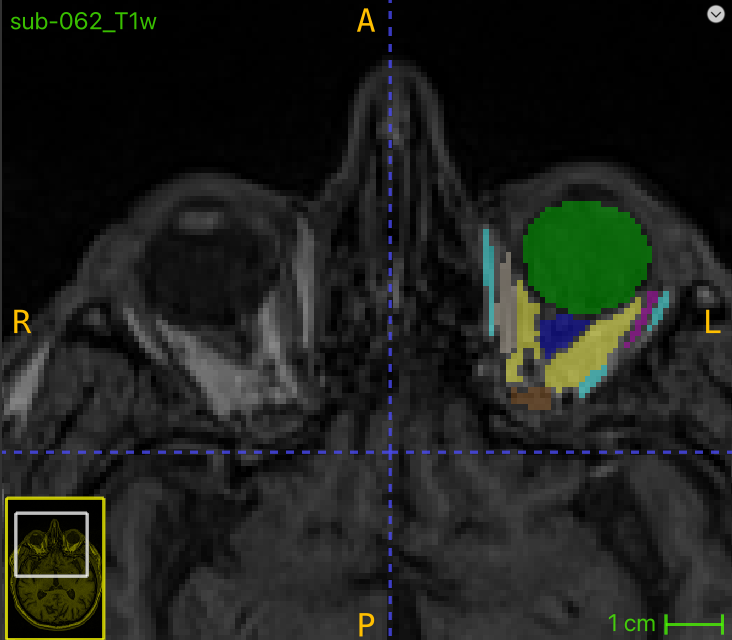
\includegraphics[width=\linewidth]{Report/img/sub-062_T1w.png}
        \caption{T1w - Subject 062}
        \label{subfig:062_T1w}
    \end{subfigure}
    \hspace{0.02\textwidth}
    \begin{subfigure}[b]{0.375\textwidth} 
        \centering
        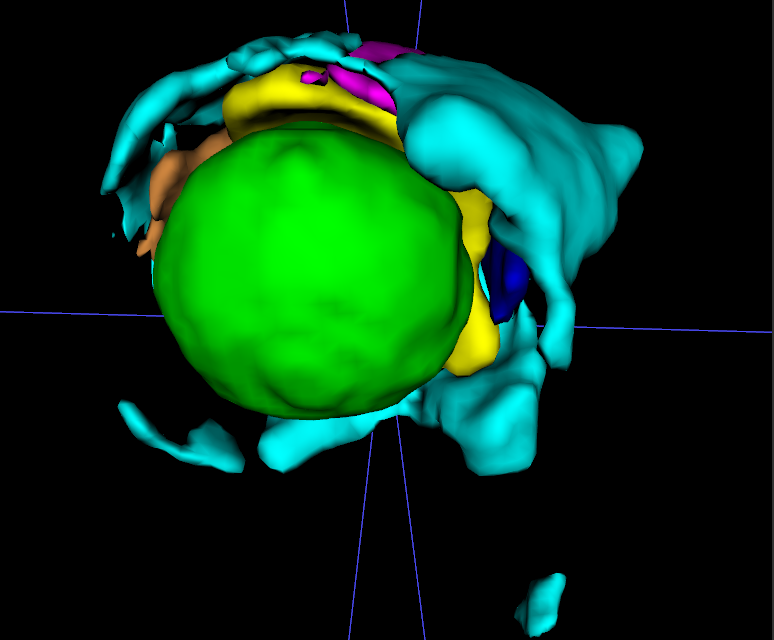
\includegraphics[width=\linewidth]{Report/img/sub-062_T1w_3D.png}
        \caption{T1w\_3D - Subject 062}
        \label{subfig:062_T1w_3D}
    \end{subfigure}

    \vspace{2mm} 

    % Second row of images
    \begin{subfigure}[b]{0.35\textwidth} 
        \centering
        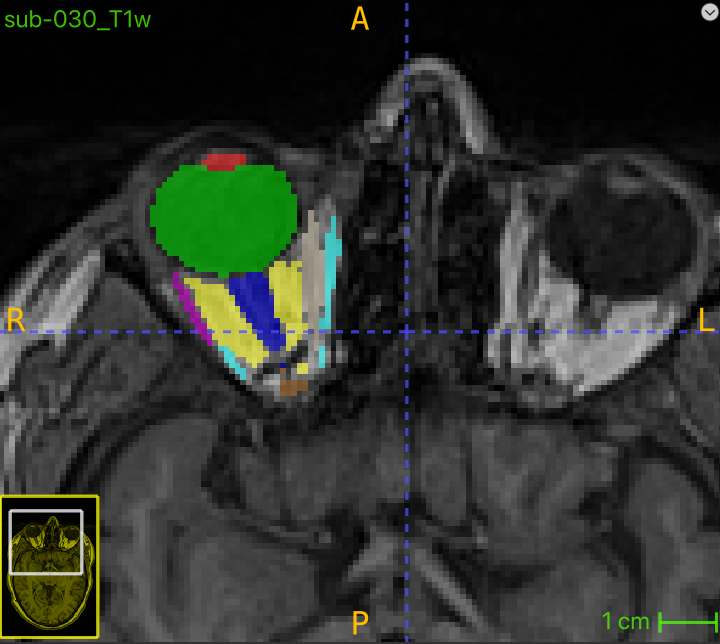
\includegraphics[width=\linewidth]{Report/img/sub-030_T1w.png}
        \caption{T1w - Subject 030}
        \label{subfig:030_T1w}
    \end{subfigure}
    \hspace{0.02\textwidth} 
    \begin{subfigure}[b]{0.375\textwidth} 
        \centering
        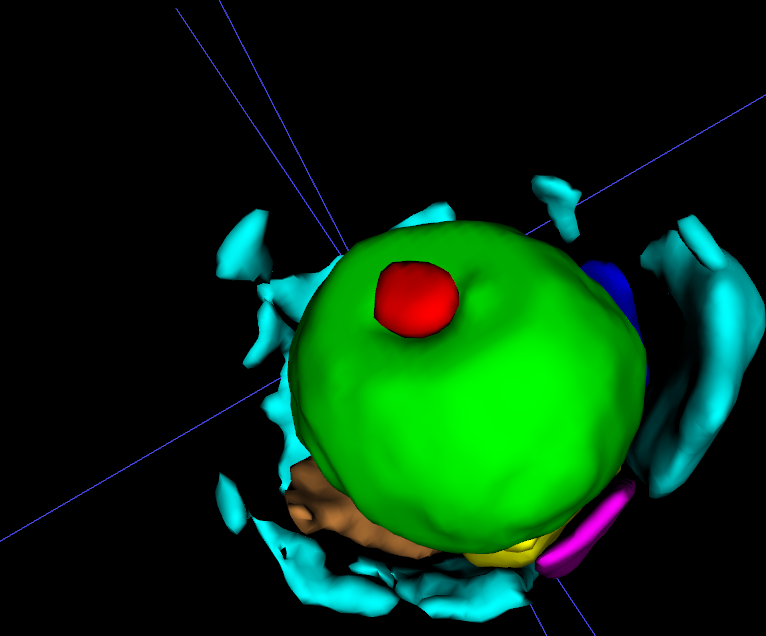
\includegraphics[width=\linewidth]{Report/img/sub-030_T1w_3D.png}
        \caption{T1w\_3D - Subject 030}
        \label{subfig:030_T1w_3D}
    \end{subfigure}
    \caption{Comparison between T1w (left column) and T1w\_3D (right column) images categorized as 'Bad' quality. These examples show noticeable but not severe blur and minor segmentation imperfections.}
    \label{fig:bad_quality_images}
\end{figure}

\subsubsection{Observation}
The 'Poor Quality' category, while also exhibiting aberrations in lens, globe, and muscle segmentations, differs from the 'Excluded' category in that these imperfections are typically isolated and less severe. Consequently, images in this category are generally still considered usable
\newpage

\subsection{Excellent Quality Images: High Fidelity}
\label{sec:excellent_quality_images}
Excellent quality images represent the ideal standard, characterized by high fidelity and clarity, making them optimal for subsequent analysis.

\begin{figure}[htbp]
    \centering
    % First row of images
    \begin{subfigure}[b]{0.35\textwidth} % Adjust subfigure width to fit content
        \centering
        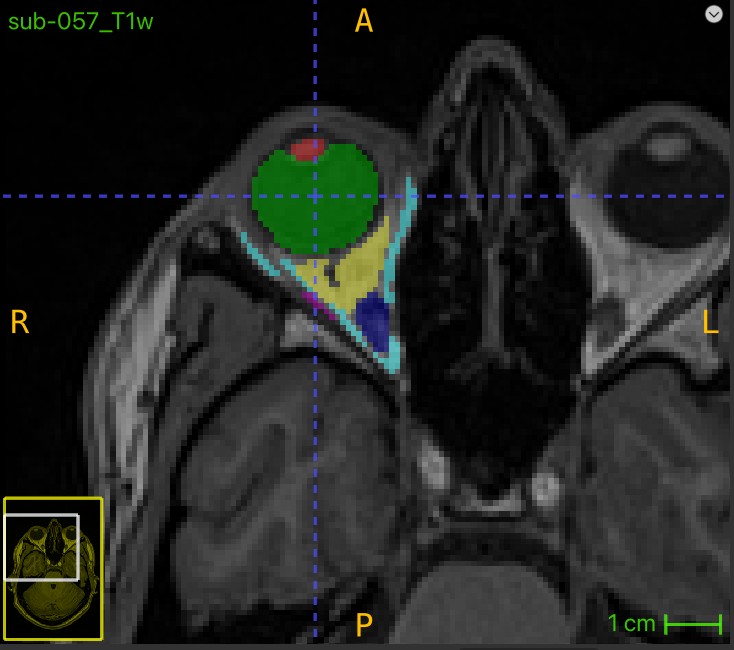
\includegraphics[width=\linewidth]{Report/img/sub-057_T1w.png}
        \caption{T1w - Subject 057}
        \label{subfig:057_T1w}
    \end{subfigure}
    \hspace{0.02\textwidth} % Small horizontal space between images
    \begin{subfigure}[b]{0.375\textwidth} % Adjust subfigure width
        \centering
        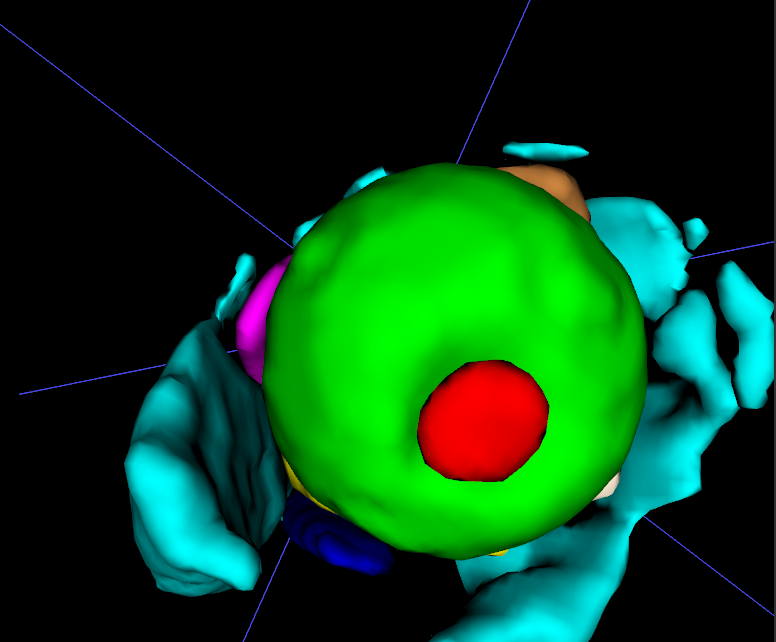
\includegraphics[width=\linewidth]{Report/img/sub-057_T1w_3D.png}
        \caption{T1w\_3D - Subject 057}
        \label{subfig:057_T1w_3D}
    \end{subfigure}

    \vspace{2mm} % Vertical space between rows

    % Second row of images
    \begin{subfigure}[b]{0.35\textwidth} % Adjust subfigure width
        \centering
        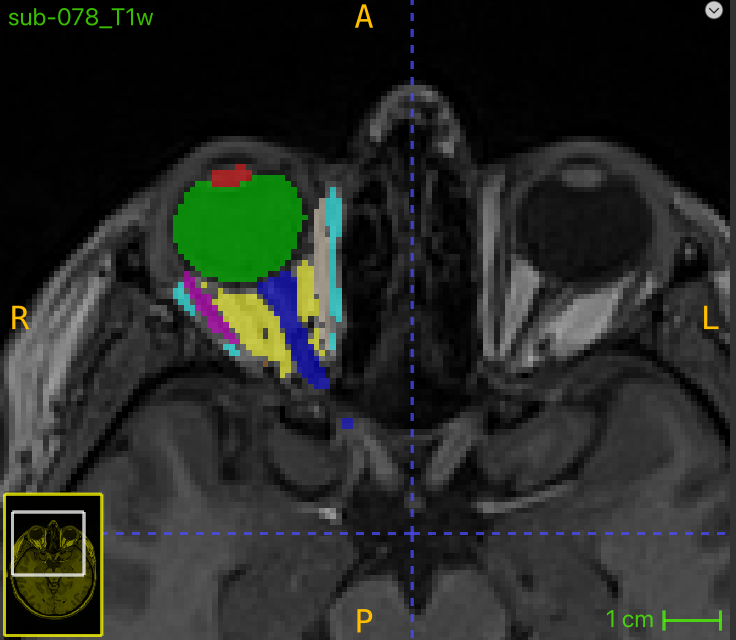
\includegraphics[width=\linewidth]{Report/img/sub-078_T1w.png}
        \caption{T1w - Subject 078}
        \label{subfig:078_T1w}
    \end{subfigure}
    \hspace{0.02\textwidth} % Small horizontal space between images
    \begin{subfigure}[b]{0.375\textwidth} % Adjust subfigure width
        \centering
        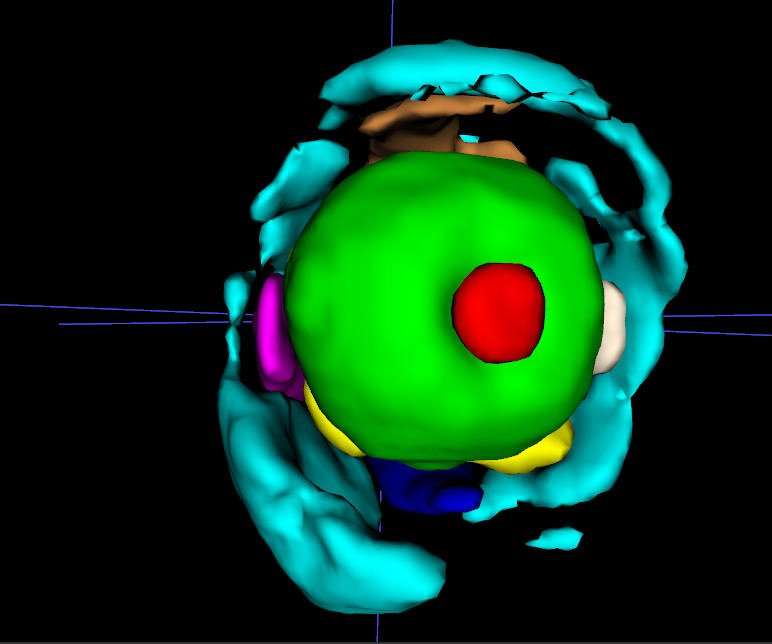
\includegraphics[width=\linewidth]{Report/img/sub-078_T1w_3D.png}
        \caption{T1w\_3D - Subject 078}
        \label{subfig:078_T1w_3D}
    \end{subfigure}
    \caption{Comparison between T1w (left column) and T1w\_3D (right column) images categorized as 'Excellent' quality. These examples showcase clear anatomical delineation, accurate segmentations, and minimal artifacts.}
    \label{fig:excellent_quality_images}
\end{figure}

\subsubsection{Observation}
Images categorized within this class are distinguished by segmentations of exceptionally high quality. Their surfaces are precisely delineated, and the morphology of the various ocular components faithfully adheres to established human anatomy. This class is notably characterized by the near-complete absence of image deterioration
\newpage
\subsection{Observations Summary for IQM Selection}
\label{sec:iqm_selection_summary}
In the segmented excluded images, the lenses exhibit distinct segmentation problems. These lenses often display discontinuous or aberrant shapes that do not correlate with the true anatomical form of a human lens, underscoring the importance of incorporating lens-segmentation-based IQMs.

Regarding the Globe, it is observable that globes in excellent quality images possess a notably smoother surface compared to those found in excluded or poor-quality images. This distinction highlights the importance of basing IQMs on this segmentation class as well.

For the other classes, no noticeable differences are consistently apparent between excluded images and excellent quality ones. This observation is attributed to the inherent complex morphology of these classes, which impedes the easy visual identification of segmentation discrepancies.